
%% bare_conf.tex
%% V1.3
%% 2007/01/11
%% by Michael Shell
%% See:
%% http://www.michaelshell.org/
%% for current contact information.
%%
%% This is a skeleton file demonstrating the use of IEEEtran.cls
%% (requires IEEEtran.cls version 1.7 or later) with an IEEE conference paper.
%%
%% Support sites:
%% http://www.michaelshell.org/tex/ieeetran/
%% http://www.ctan.org/tex-archive/macros/latex/contrib/IEEEtran/
%% and
%% http://www.ieee.org/

%%*************************************************************************
%% Legal Notice:
%% This code is offered as-is without any warranty either expressed or
%% implied; without even the implied warranty of MERCHANTABILITY or
%% FITNESS FOR A PARTICULAR PURPOSE! 
%% User assumes all risk.
%% In no event shall IEEE or any contributor to this code be liable for
%% any damages or losses, including, but not limited to, incidental,
%% consequential, or any other damages, resulting from the use or misuse
%% of any information contained here.
%%
%% All comments are the opinions of their respective authors and are not
%% necessarily endorsed by the IEEE.
%%
%% This work is distributed under the LaTeX Project Public License (LPPL)
%% ( http://www.latex-project.org/ ) version 1.3, and may be freely used,
%% distributed and modified. A copy of the LPPL, version 1.3, is included
%% in the base LaTeX documentation of all distributions of LaTeX released
%% 2003/12/01 or later.
%% Retain all contribution notices and credits.
%% ** Modified files should be clearly indicated as such, including  **
%% ** renaming them and changing author support contact information. **
%%
%% File list of work: IEEEtran.cls, IEEEtran_HOWTO.pdf, bare_adv.tex,
%%                    bare_conf.tex, bare_jrnl.tex, bare_jrnl_compsoc.tex
%%*************************************************************************

% *** Authors should verify (and, if needed, correct) their LaTeX system  ***
% *** with the testflow diagnostic prior to trusting their LaTeX platform ***
% *** with production work. IEEE's font choices can trigger bugs that do  ***
% *** not appear when using other class files.                            ***
% The testflow support page is at:
% http://www.michaelshell.org/tex/testflow/



% Note that the a4paper option is mainly intended so that authors in
% countries using A4 can easily print to A4 and see how their papers will
% look in print - the typesetting of the document will not typically be
% affected with changes in paper size (but the bottom and side margins will).
% Use the testflow package mentioned above to verify correct handling of
% both paper sizes by the user's LaTeX system.
%
% Also note that the "draftcls" or "draftclsnofoot", not "draft", option
% should be used if it is desired that the figures are to be displayed in
% draft mode.
%
\documentclass[conference]{IEEEtran}
% Add the compsoc option for Computer Society conferences.
%
% If IEEEtran.cls has not been installed into the LaTeX system files,
% manually specify the path to it like:
% \documentclass[conference]{../sty/IEEEtran}





% Some very useful LaTeX packages include:
% (uncomment the ones you want to load)


% *** MISC UTILITY PACKAGES ***
%
%\usepackage{ifpdf}
% Heiko Oberdiek's ifpdf.sty is very useful if you need conditional
% compilation based on whether the output is pdf or dvi.
% usage:
% \ifpdf
%   % pdf code
% \else
%   % dvi code
% \fi
% The latest version of ifpdf.sty can be obtained from:
% http://www.ctan.org/tex-archive/macros/latex/contrib/oberdiek/
% Also, note that IEEEtran.cls V1.7 and later provides a builtin
% \ifCLASSINFOpdf conditional that works the same way.
% When switching from latex to pdflatex and vice-versa, the compiler may
% have to be run twice to clear warning/error messages.






% *** CITATION PACKAGES ***
%
%\usepackage{cite}
% cite.sty was written by Donald Arseneau
% V1.6 and later of IEEEtran pre-defines the format of the cite.sty package
% \cite{} output to follow that of IEEE. Loading the cite package will
% result in citation numbers being automatically sorted and properly
% "compressed/ranged". e.g., [1], [9], [2], [7], [5], [6] without using
% cite.sty will become [1], [2], [5]--[7], [9] using cite.sty. cite.sty's
% \cite will automatically add leading space, if needed. Use cite.sty's
% noadjust option (cite.sty V3.8 and later) if you want to turn this off.
% cite.sty is already installed on most LaTeX systems. Be sure and use
% version 4.0 (2003-05-27) and later if using hyperref.sty. cite.sty does
% not currently provide for hyperlinked citations.
% The latest version can be obtained at:
% http://www.ctan.org/tex-archive/macros/latex/contrib/cite/
% The documentation is contained in the cite.sty file itself.






% *** GRAPHICS RELATED PACKAGES ***
%
\ifCLASSINFOpdf
   \usepackage[pdftex]{graphicx}
  % declare the path(s) where your graphic files are
   \graphicspath{{../pdf/}{../jpeg/}}
  % and their extensions so you won't have to specify these with
  % every instance of \includegraphics
   \DeclareGraphicsExtensions{.pdf,.jpeg,.png}
\else
  % or other class option (dvipsone, dvipdf, if not using dvips). graphicx
  % will default to the driver specified in the system graphics.cfg if no
  % driver is specified.
   \usepackage[dvips]{graphicx}
  % declare the path(s) where your graphic files are
   \graphicspath{{./}}
  % and their extensions so you won't have to specify these with
  % every instance of \includegraphics
%   \DeclareGraphicsExtensions{.eps}
\fi
% graphicx was written by David Carlisle and Sebastian Rahtz. It is
% required if you want graphics, photos, etc. graphicx.sty is already
% installed on most LaTeX systems. The latest version and documentation can
% be obtained at: 
% http://www.ctan.org/tex-archive/macros/latex/required/graphics/
% Another good source of documentation is "Using Imported Graphics in
% LaTeX2e" by Keith Reckdahl which can be found as epslatex.ps or
% epslatex.pdf at: http://www.ctan.org/tex-archive/info/
%
% latex, and pdflatex in dvi mode, support graphics in encapsulated
% postscript (.eps) format. pdflatex in pdf mode supports graphics
% in .pdf, .jpeg, .png and .mps (metapost) formats. Users should ensure
% that all non-photo figures use a vector format (.eps, .pdf, .mps) and
% not a bitmapped formats (.jpeg, .png). IEEE frowns on bitmapped formats
% which can result in "jaggedy"/blurry rendering of lines and letters as
% well as large increases in file sizes.
%
% You can find documentation about the pdfTeX application at:
% http://www.tug.org/applications/pdftex


\usepackage{epstopdf}


% *** MATH PACKAGES ***
%
\usepackage[cmex10]{amsmath}
% A popular package from the American Mathematical Society that provides
% many useful and powerful commands for dealing with mathematics. If using
% it, be sure to load this package with the cmex10 option to ensure that
% only type 1 fonts will utilized at all point sizes. Without this option,
% it is possible that some math symbols, particularly those within
% footnotes, will be rendered in bitmap form which will result in a
% document that can not be IEEE Xplore compliant!
%
% Also, note that the amsmath package sets \interdisplaylinepenalty to 10000
% thus preventing page breaks from occurring within multiline equations. Use:
%\interdisplaylinepenalty=2500
% after loading amsmath to restore such page breaks as IEEEtran.cls normally
% does. amsmath.sty is already installed on most LaTeX systems. The latest
% version and documentation can be obtained at:
% http://www.ctan.org/tex-archive/macros/latex/required/amslatex/math/





% *** SPECIALIZED LIST PACKAGES ***
%
%\usepackage{algorithmic}
% algorithmic.sty was written by Peter Williams and Rogerio Brito.
% This package provides an algorithmic environment fo describing algorithms.
% You can use the algorithmic environment in-text or within a figure
% environment to provide for a floating algorithm. Do NOT use the algorithm
% floating environment provided by algorithm.sty (by the same authors) or
% algorithm2e.sty (by Christophe Fiorio) as IEEE does not use dedicated
% algorithm float types and packages that provide these will not provide
% correct IEEE style captions. The latest version and documentation of
% algorithmic.sty can be obtained at:
% http://www.ctan.org/tex-archive/macros/latex/contrib/algorithms/
% There is also a support site at:
% http://algorithms.berlios.de/index.html
% Also of interest may be the (relatively newer and more customizable)
% algorithmicx.sty package by Szasz Janos:
% http://www.ctan.org/tex-archive/macros/latex/contrib/algorithmicx/




% *** ALIGNMENT PACKAGES ***
%
%\usepackage{array}
% Frank Mittelbach's and David Carlisle's array.sty patches and improves
% the standard LaTeX2e array and tabular environments to provide better
% appearance and additional user controls. As the default LaTeX2e table
% generation code is lacking to the point of almost being broken with
% respect to the quality of the end results, all users are strongly
% advised to use an enhanced (at the very least that provided by array.sty)
% set of table tools. array.sty is already installed on most systems. The
% latest version and documentation can be obtained at:
% http://www.ctan.org/tex-archive/macros/latex/required/tools/


%\usepackage{mdwmath}
%\usepackage{mdwtab}
% Also highly recommended is Mark Wooding's extremely powerful MDW tools,
% especially mdwmath.sty and mdwtab.sty which are used to format equations
% and tables, respectively. The MDWtools set is already installed on most
% LaTeX systems. The lastest version and documentation is available at:
% http://www.ctan.org/tex-archive/macros/latex/contrib/mdwtools/


% IEEEtran contains the IEEEeqnarray family of commands that can be used to
% generate multiline equations as well as matrices, tables, etc., of high
% quality.


%\usepackage{eqparbox}
% Also of notable interest is Scott Pakin's eqparbox package for creating
% (automatically sized) equal width boxes - aka "natural width parboxes".
% Available at:
% http://www.ctan.org/tex-archive/macros/latex/contrib/eqparbox/





% *** SUBFIGURE PACKAGES ***
%\usepackage[tight,footnotesize]{subfigure}
% subfigure.sty was written by Steven Douglas Cochran. This package makes it
% easy to put subfigures in your figures. e.g., "Figure 1a and 1b". For IEEE
% work, it is a good idea to load it with the tight package option to reduce
% the amount of white space around the subfigures. subfigure.sty is already
% installed on most LaTeX systems. The latest version and documentation can
% be obtained at:
% http://www.ctan.org/tex-archive/obsolete/macros/latex/contrib/subfigure/
% subfigure.sty has been superceeded by subfig.sty.



%\usepackage[caption=false]{caption}
%\usepackage[font=footnotesize]{subfig}
% subfig.sty, also written by Steven Douglas Cochran, is the modern
% replacement for subfigure.sty. However, subfig.sty requires and
% automatically loads Axel Sommerfeldt's caption.sty which will override
% IEEEtran.cls handling of captions and this will result in nonIEEE style
% figure/table captions. To prevent this problem, be sure and preload
% caption.sty with its "caption=false" package option. This is will preserve
% IEEEtran.cls handing of captions. Version 1.3 (2005/06/28) and later 
% (recommended due to many improvements over 1.2) of subfig.sty supports
% the caption=false option directly:
%\usepackage[caption=false,font=footnotesize]{subfig}
%
% The latest version and documentation can be obtained at:
% http://www.ctan.org/tex-archive/macros/latex/contrib/subfig/
% The latest version and documentation of caption.sty can be obtained at:
% http://www.ctan.org/tex-archive/macros/latex/contrib/caption/




% *** FLOAT PACKAGES ***
%
%\usepackage{fixltx2e}
% fixltx2e, the successor to the earlier fix2col.sty, was written by
% Frank Mittelbach and David Carlisle. This package corrects a few problems
% in the LaTeX2e kernel, the most notable of which is that in current
% LaTeX2e releases, the ordering of single and double column floats is not
% guaranteed to be preserved. Thus, an unpatched LaTeX2e can allow a
% single column figure to be placed prior to an earlier double column
% figure. The latest version and documentation can be found at:
% http://www.ctan.org/tex-archive/macros/latex/base/



%\usepackage{stfloats}
% stfloats.sty was written by Sigitas Tolusis. This package gives LaTeX2e
% the ability to do double column floats at the bottom of the page as well
% as the top. (e.g., "\begin{figure*}[!b]" is not normally possible in
% LaTeX2e). It also provides a command:
%\fnbelowfloat
% to enable the placement of footnotes below bottom floats (the standard
% LaTeX2e kernel puts them above bottom floats). This is an invasive package
% which rewrites many portions of the LaTeX2e float routines. It may not work
% with other packages that modify the LaTeX2e float routines. The latest
% version and documentation can be obtained at:
% http://www.ctan.org/tex-archive/macros/latex/contrib/sttools/
% Documentation is contained in the stfloats.sty comments as well as in the
% presfull.pdf file. Do not use the stfloats baselinefloat ability as IEEE
% does not allow \baselineskip to stretch. Authors submitting work to the
% IEEE should note that IEEE rarely uses double column equations and
% that authors should try to avoid such use. Do not be tempted to use the
% cuted.sty or midfloat.sty packages (also by Sigitas Tolusis) as IEEE does
% not format its papers in such ways.





% *** PDF, URL AND HYPERLINK PACKAGES ***
%
%\usepackage{url}
% url.sty was written by Donald Arseneau. It provides better support for
% handling and breaking URLs. url.sty is already installed on most LaTeX
% systems. The latest version can be obtained at:
% http://www.ctan.org/tex-archive/macros/latex/contrib/misc/
% Read the url.sty source comments for usage information. Basically,
% \url{my_url_here}.





% *** Do not adjust lengths that control margins, column widths, etc. ***
% *** Do not use packages that alter fonts (such as pslatex).         ***
% There should be no need to do such things with IEEEtran.cls V1.6 and later.
% (Unless specifically asked to do so by the journal or conference you plan
% to submit to, of course. )


% correct bad hyphenation here
\hyphenation{op-tical net-works semi-conduc-tor}


\begin{document}
%
% paper title
% can use linebreaks \\ within to get better formatting as desired
\title{Motor Experience Alters Action Perception Through Predictive Learning of Sensorimotor Information}

% author names and affiliations
% use a multiple column layout for up to three different
% affiliations
\author{\IEEEauthorblockN{Jimmy Baraglia, Jorge L. Copete, Yukie Nagai, and Minoru Asada}
\IEEEauthorblockA{Graduate School of Engineering, Osaka University\\
2-1 Yamada-oka, Suita, Osaka, 565-0871 Japan \\
Email:  \{jimmy.baraglia,jorge.copete,yukie,asada\}@ams.eng.osaka-u.ac.jp}
%\and
%\IEEEauthorblockN{Homer Simpson}
%\IEEEauthorblockA{Twentieth Century Fox\\
%Springfield, USA\\
%Email: homer@thesimpsons.com}
}

% conference papers do not typically use \thanks and this command
% is locked out in conference mode. If really needed, such as for
% the acknowledgment of grants, issue a \IEEEoverridecommandlockouts
% after \documentclass

% for over three affiliations, or if they all won't fit within the width
% of the page, use this alternative format:
% 
%\author{\IEEEauthorblockN{Michael Shell\IEEEauthorrefmark{1},
%Homer Simpson\IEEEauthorrefmark{2},
%James Kirk\IEEEauthorrefmark{3}, 
%Montgomery Scott\IEEEauthorrefmark{3} and
%Eldon Tyrell\IEEEauthorrefmark{4}}
%\IEEEauthorblockA{\IEEEauthorrefmark{1}School of Electrical and Computer Engineering\\
%Georgia Institute of Technology,
%Atlanta, Georgia 30332--0250\\ Email: see http://www.michaelshell.org/contact.html}
%\IEEEauthorblockA{\IEEEauthorrefmark{2}Twentieth Century Fox, Springfield, USA\\
%Email: homer@thesimpsons.com}
%\IEEEauthorblockA{\IEEEauthorrefmark{3}Starfleet Academy, San Francisco, California 96678-2391\\
%Telephone: (800) 555--1212, Fax: (888) 555--1212}
%\IEEEauthorblockA{\IEEEauthorrefmark{4}Tyrell Inc., 123 Replicant Street, Los Angeles, California 90210--4321}}




% use for special paper notices
%\IEEEspecialpapernotice{(Invited Paper)}


% make the title area
\maketitle

\begin{abstract}
%\boldmath
Recent studies have revealed that infants' goal-directed action execution strongly alters their perception of similar actions performed by other individuals. Such an ability to recognize correspondences between self-experience and others' actions may be crucial for the development of higher cognitive social skills. However, there is not yet a computational model or constructive explanation accounting for the role of action generation in the perception of others' actions. To address this issue, we hypothesize that the sensory and motor information are integrated at a neural level through a predictive learning process. Thus, the experience of motor actions alters the representation of the sensorimotor integration, which causes changes in the perception of others' actions. To test this hypothesis, we built a computational model that integrates visual and motor (hereafter, visuomotor) information using a Recurrent Neural Network (RNN) which is capable of learning temporal sequences of data. We modeled the visual attention of the system based on a prediction error between the sensory prediction and the actual sensory values, which maximizes the attention toward not too predictable and not too unpredictable sensory information. We performed a series of experiments with a simulated humanoid robot from which we observed that motor activation during self-generated actions biased the robot's perception of others' actions. These results highlight the important role of modalities integration in humans, which accounts for a biased perception of our environment based on a restricted repertoire of own experienced actions.

\end{abstract}
% IEEEtran.cls defaults to using nonbold math in the Abstract.
% This preserves the distinction between vectors and scalars. However,
% if the conference you are submitting to favors bold math in the abstract,
% then you can use LaTeX's standard command \boldmath at the very start
% of the abstract to achieve this. Many IEEE journals/conferences frown on
% math in the abstract anyway.

% no keywords

% For peer review papers, you can put extra information on the cover
% page as needed:
% \ifCLASSOPTIONpeerreview
% \begin{center} \bfseries EDICS Category: 3-BBND \end{center}
% \fi
%
% For peerreview papers, this IEEEtran command inserts a page break and
% creates the second title. It will be ignored for other modes.
\IEEEpeerreviewmaketitle


\section{Introduction}
% no \IEEEPARstart
In early infancy, humans are not yet able to detect the goal of others' actions. Later on, infants undergo a developmental process that allows them to perceive others' actions as goal-directed. Several studies have been carried out to reveal when and how infants start understanding goal-directed actions. A remarkable work conducted by Woodward \cite{woodward1998infants} shows that infants (5, 6 and 9 months old) with goal-directed action experience react differently to actors reaching for and grasping objects. For the experiments four actors were presented to the infants: a human arm, a rod, a flat occluder and a mechanical grasping tool. The experiment indicated that when infants were habituated to goal-directed actions (i.e., the human arm condition) they showed a stronger novelty response to test events that varied the goal of the action (e.g., the grasped object) than test events that varied the physical properties of the action (e.g., the motion path). On the other hand, if the actions were not goal-directed (i.e., the rod and the flat occluder conditions), or were goal-directed but difficult to infer the agency of the actor (i.e., the mechanical grasping tool condition), infants did not prefer one type of response to the other (i.e., the goal of the action versus the properties of the action).

Later, Sommerville et al. \cite{sommerville2005action} studied the impact of infants' action production in perception of others' actions. The participants of the experiment were 3-month-old infants. They were divided in two groups. The first group of infants participated in an action task which consisted in interacting with two objects in order to acquire action experience. Due to the fact that 3-month-old infants are not yet able to perform coordinated gaze and manual contact with objects, they put a pair of mittens on the infants' hands so that they can easily make contact with them. The second group did not participate in the action task. Then, during the habituation phase, both groups of infants saw an actor reaching for and grasping one of two objects. Finally, during the test phase, the position of the objects was reversed and the infants saw new test events: a new goal event (i.e., the actor reached the same position as habituation but grasped a different goal), and a new path event (i.e., the actor reached a different position but grasped the same goal). Infants' looking time was measured during the experiment. The results showed that the looking time of the first group of infants was longer than the looking time of the second group in the first trial of the habituation phase. Also, the first group of infants looked significantly longer at the new goal event than the new path event, whereas the second group of infants looked equally to both events. According to Sommerville et al. \cite{sommerville2005action}, these findings reflect infants’ ability to detect the goal structure of action after experiencing object-directed behavior, and to apply this knowledge when perceiving others' actions. Therefore, in order to understand this phenomenon, we find important to clarify the underlying mechanism that accounts for the influence of the motor system on the perceptual system and enables infants to detect the goal in others' actions. Further, we need to explain the connection of this mechanism to the visual attention, in accordance to \cite{sommerville2005action} which found that self-action production leads to an increase of visual attention to action goals. In regard to studies on visual attention, experiments conducted by Kidd et al. \cite{kidd2012goldilocks} showed that, when varying the complexity of a sequence of visual events, the probability of infants (7- and 8-month-old) to look away from those events became higher when the complexity of the stimulus was very low or very high. Their findings suggested that infants allocate their attention in order to maintain an intermediate level of complexity.

In this study we build a computational model to explain how action production alters perception of others’ actions as reported by Sommerville et al. \cite{sommerville2005action}. Specifically, we focus on the relation between the visual and motor systems and the effect of action experience on the perception of others' actions. Our hypothesis is that motor activity biases visual perception through the joint representation of visuomotor experiences. As an extension to the aforementioned hypothesis, we also propose that the allocation of visual attention is modulated by the prediction error that results from making correspondence between own experience and others' actions. We carried out experiments using iCub Simulator to validate our hypothesis.

\section{Hypothesis}
 
\subsection{Findings in Infant Study}
Sommerville et al. \cite{sommerville2005action} reported that infants' action experience alters their perception when observing others' actions. Here we focused on two main findings:
 
\begin{enumerate}
\item Experience apprehending objects initially increases infants' attention to similar reaching events performed by another person (Figure 2 in \cite{sommerville2005action});
\item Infants with apprehension experience look significantly longer at new goal events than new path events, whereas infants without that experience looked equally to both events (Figure 3 in \cite{sommerville2005action}).
\end{enumerate}
 
Sommerville et al. \cite{sommerville2005action} suggested that the first finding "may reflect infants’ ability to recognize correspondences across executed and observed actions and/or an increased motivation to attend to action after acting". Regarding the second finding, they indicated that "experience apprehending objects directly prior to viewing the visual habituation event enabled infants to detect the goal-directed structure of the event in another person's actions".

\subsection{Our Hypothesis}
We argue that action experience is acquired through the process of integrating motor and sensory information, and that the joint representation derived from this integration is used to learn to predict other's actions. Further, the motor information contains a representation of the action goal that alters the sensorimotor representation in terms of the goal \cite{rizzolatti2014cortical}, and that is how the motor experience allows infants to detect the goal in others' actions. Based on this argumentation, our hypothesis is that when perceiving others' actions infants make predictions based on the sensory information (Fig. \ref{Hypothesis}-a), whereas when generating actions infants learn to predict motor and sensory information, and consequently to encode the sensorimotor representation of experiences in terms of goals (Fig. \ref{Hypothesis}-b). Therefore, since both action perception and action production share the same predictor, then action production has influence on action observation.

\begin{figure}[!t]
\centering
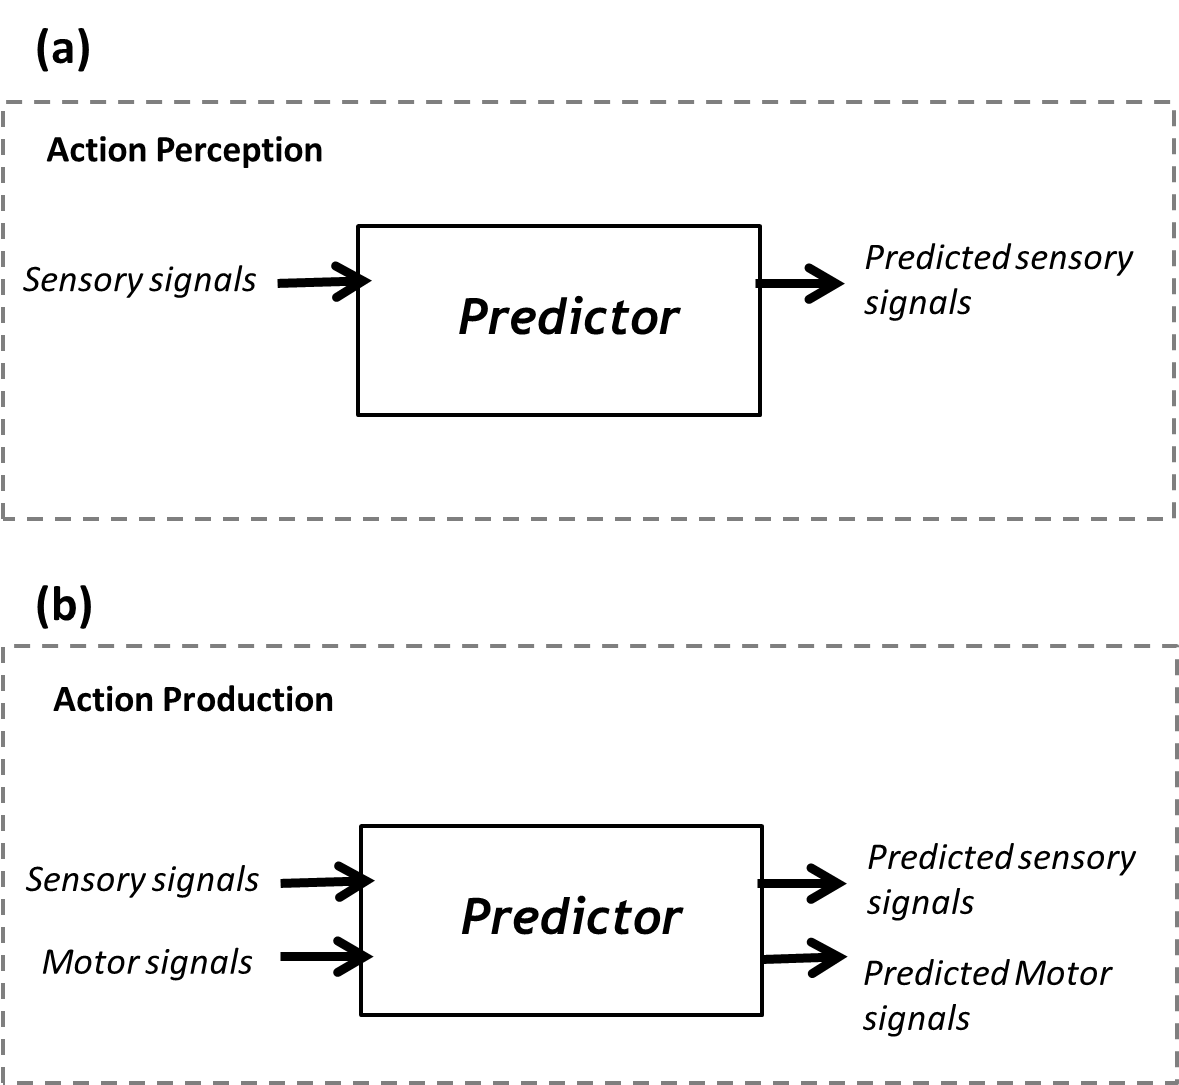
\includegraphics[width=0.5\textwidth,natwidth=700,natheight=450]{Hypothesis.png}
\caption{Our hypothesis. (a) During the action observation infants receive sensory information and predict sensory information. (b) During the action observation infants receive sensory and motor information and predict sensory and motor information.}
\label{Hypothesis}
\end{figure}

During this learning process a prediction error arises between the predicted sensory information and the actual one. The magnitude of the prediction error depends on the action experience. We argue that the prediction error plays a fundamental role in the development of several cognitive abilities \cite{nagai2015}. Kilner et al. \cite{kilner2007predictive} showed that prediction error could account for the development of the mirror neuron systems. Their hypothesis is that minimizing the prediction error could help inferring the cause of an observed action. Furthermore, based on the development of attention and the mirror neuron system, several robotic studies propose that predictive learning could also account for the development of imitation \cite{minato2010model}, helping behavior \cite{baraglia2014prediction} and goal-directed prediction in early infancy \cite{copete2014development}. Here, we hypothesize that the prediction error modulates the level of attention to external stimulus through an interest function  \cite{nagai2015}, as shown in Fig. \ref{Attention}. We support our idea based on evidence in \cite{kidd2012goldilocks} according to which visual allocation depends on the complexity of the events, where scenes of middle level complexity draw more attention than those of low and high levels. Thus, the prediction error accounts for the complexity of an event.

\begin{figure}[!t]
\centering
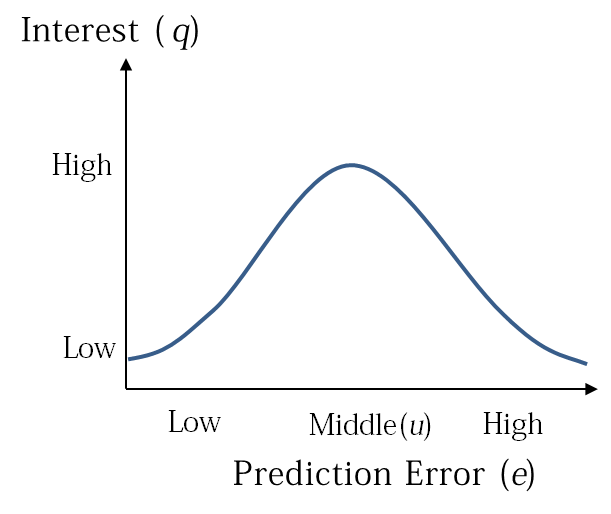
\includegraphics[width=0.3\textwidth,natwidth=700,natheight=450]{Figure5.png}
\caption{Visual attention. Curve of interest value in function of the prediction error.}
\label{Attention}
\end{figure}

We explain findings in \cite{sommerville2005action} in correspondence to our hypothesis by saying that the motor information when infants produce actions changes the sensorimotor representation used to predict sensory information from new events. Then, for the first finding (subsection A-1), we argue that the action experience makes others' actions become more predictable although not completely predictable, which generates an error in the prediction that changes infants' attention. For the second finding (subsection A-2), we say that the action experience enables infants to make predictions based more on the goal than on the trajectory due to the influence of the motor signal, which produces a change in the visual attention as a function of the prediction error. This underline the important role of the motor signal representing action goals.

\section{Computational Model}
We propose a computational model based on our hypothesis which consists of four modules: the visual module, the motor module, the sensorimotor integration, and the visual attention module. The details of each module are explained in following subsections.

\subsection{Motor Module}
The motor module generates motor activation signals when the system performs actions. Here, we represent the motor activity as a distinctive set of signals which encode the target of the action and the motor primitive currently generated. This module will output:
\begin{itemize}
\item the motor primitives \(\text{P}=[\textit{p}_{1},...,\textit{p}_{m}]\) represented as a vector of $m$ binary signals whose components take values 0 or 1, where $m$ is the number of action primitives,
\item and the target of the ongoing action \(\text{G}=[\textit{g}_{1},...,\textit{g}_{n}]\) as a vector of $n$ binary and mutually exclusive signals whose components take values 0 or 1, where $n$ is the number of target objects in the scene.
\end{itemize}
For the case of two objects ($n$=2) and two motor primitives ($m$=2): arm reaching primitive and arm retracting primitive, the motor module will output a vector \textbf{M} composed of four activation signals,
\begin{equation}
	\textbf{M}(t)=[\textit{g}_{1}(t), \textit{g}_{2}(t), \textit{p}_{1}(t), \textit{p}_{2}(t)],
\end{equation}
where $t$ represents the time. The choice of variables is based on the idea that infants' actions are goal directed (see goal babbling theory \cite{rolf2012goal}). Thus, it is important to represent both the motion primitives used to perform an action and the targets (goals).

\subsection{Vision Module}
The vision module extracts visual information when the system observes actions and then provides the position of the moving effector and the relations between objects in the scene. To do so, the module first extracts and tracks the objects in the scene, then measures the dynamic of the moving effector relative to the objects and finally employs the resulting motion vectors to calculate their relations. Here relations refer to the relative dynamic between objects and the moving effector. For example the moving effector getting closer to (or getting away from) an object is considered a relation. This module will output:
\begin{itemize}
\item the position [$x$, $y$, $z$] of the moving effector,
\item the vector \(\textbf{R}=[\textit{r}_{11},...,\textit{r}_{1s},...,\text{r}_{n1},...,\textit{r}_{ns}]\) of \(s \times n\) possible combinations between the moving effector and $n$ objects for $s$ relations, whose components take values 0 or 1,
\item and the vector \(\textbf{RG}=[\textit{rg}_{1},...,\textit{rg}_{s}]\) of $s$ possible relations between the moving effector and any object, whose components take values 0 or 1.
\end{itemize}

This choice is justified by the fact that infants can be expected to distinguish between objects and actors (see \cite{woodward1998infants}), and therefore to be potentially able to recognize dynamic relations between them. Note that visual relations contained in the vector $\textbf{R}$ are dependent on the identity of the objects regardless of their positions, while the relations contained in the vector $\textbf{RG}$ takes accounts all the objects for each relation (e.g., the relation getting closer takes value 1 if the moving effector is getting closer to any object), which guarantees a differentiated representation of the dynamic of the moving effector regardless of the identity of the targeted object.

Thus, for the case of two objects ($n$=2) and two relations ($s$=2), getting closer and getting away, the vision module will output a vector \(\textbf{V}\) made of nine signals,
\begin{equation}
\begin{split}
	\textbf{V}(t)=[\textit{x}(t), \textit{y}(t), \textit{z}(t), \textit{r}_{11}(t), \textit{r}_{12}(t),\\ \textit{r}_{21}(t), \textit{r}_{22}(t), \textit{rg}_{1}(t), \textit{rg}_{2}(t)],
\end{split}
\end{equation}

\subsection{Sensorimotor Integration Module}
\subsubsection{Sensorimotor Integration}
Biological systems use multiple sensorimotor modalities to interact with their environment. In this with this, studies in robotics have adopted multi-modal integration approaches to model multiple behavior patterns using visuomotor information \cite{noda2014multimodal}. We argue that the process of integrating multi-modal information, such as visual and motor information, encodes our experience and is vital to understand others' action goals. Another related aspect is that humans tend to anticipate near future events when interacting with their environment based on the sensory data they perceive \cite{cannon2012infants}. Recent studies have shown that predictive learning is important to shape infants' perception of the world and direct their attention model \cite{den2012prediction}. Here, we take advantage of the structure and functionality of the Elman Recurrent Neural Network (RNN) \cite{elman1990finding} which can perform integration of multiple data and learn the characteristics of temporal sequence data. The model of the neural network is shown in Fig. \ref{NeuralNet}. The inputs of the neural network \(\textbf{I}(t)\) are the outputs from the visual module and the motor module. We used 13 neurons in the input and output units, and 50 neurons in the hidden and context units, which was empirically decided as the minimum number of neurons for the network to converge.

\begin{equation}
	\textbf{I}(t)=[\textbf{V}(t), \textbf{M}(t)],\\
\end{equation}
and the outputs \(\textbf{O}(t)\) are the predicted visual and motor data,
\begin{equation}
	\textbf{O}(t+1)=[\hat{\textbf{V}}(t+1), \hat{\textbf{M}}(t+1)],\\
\end{equation}
where \(\hat{\textbf{V}}(t+1)\) is the predicted visual information, and  \(\hat{\textbf{M}}(t+1)\) is the predicted motor information. The internal composition of \(\hat{\textbf{V}}(t+1)\) and \(\hat{\textbf{M}}(t+1)\) is equivalent to \(\text{\textbf{V}}(t)\) and \(\text{\textbf{M}}(t)\), respectively. The neural network is trained using the back propagation through time method to minimize the learning error which includes visual and motor prediction errors.

\begin{figure}[!t]
\centering
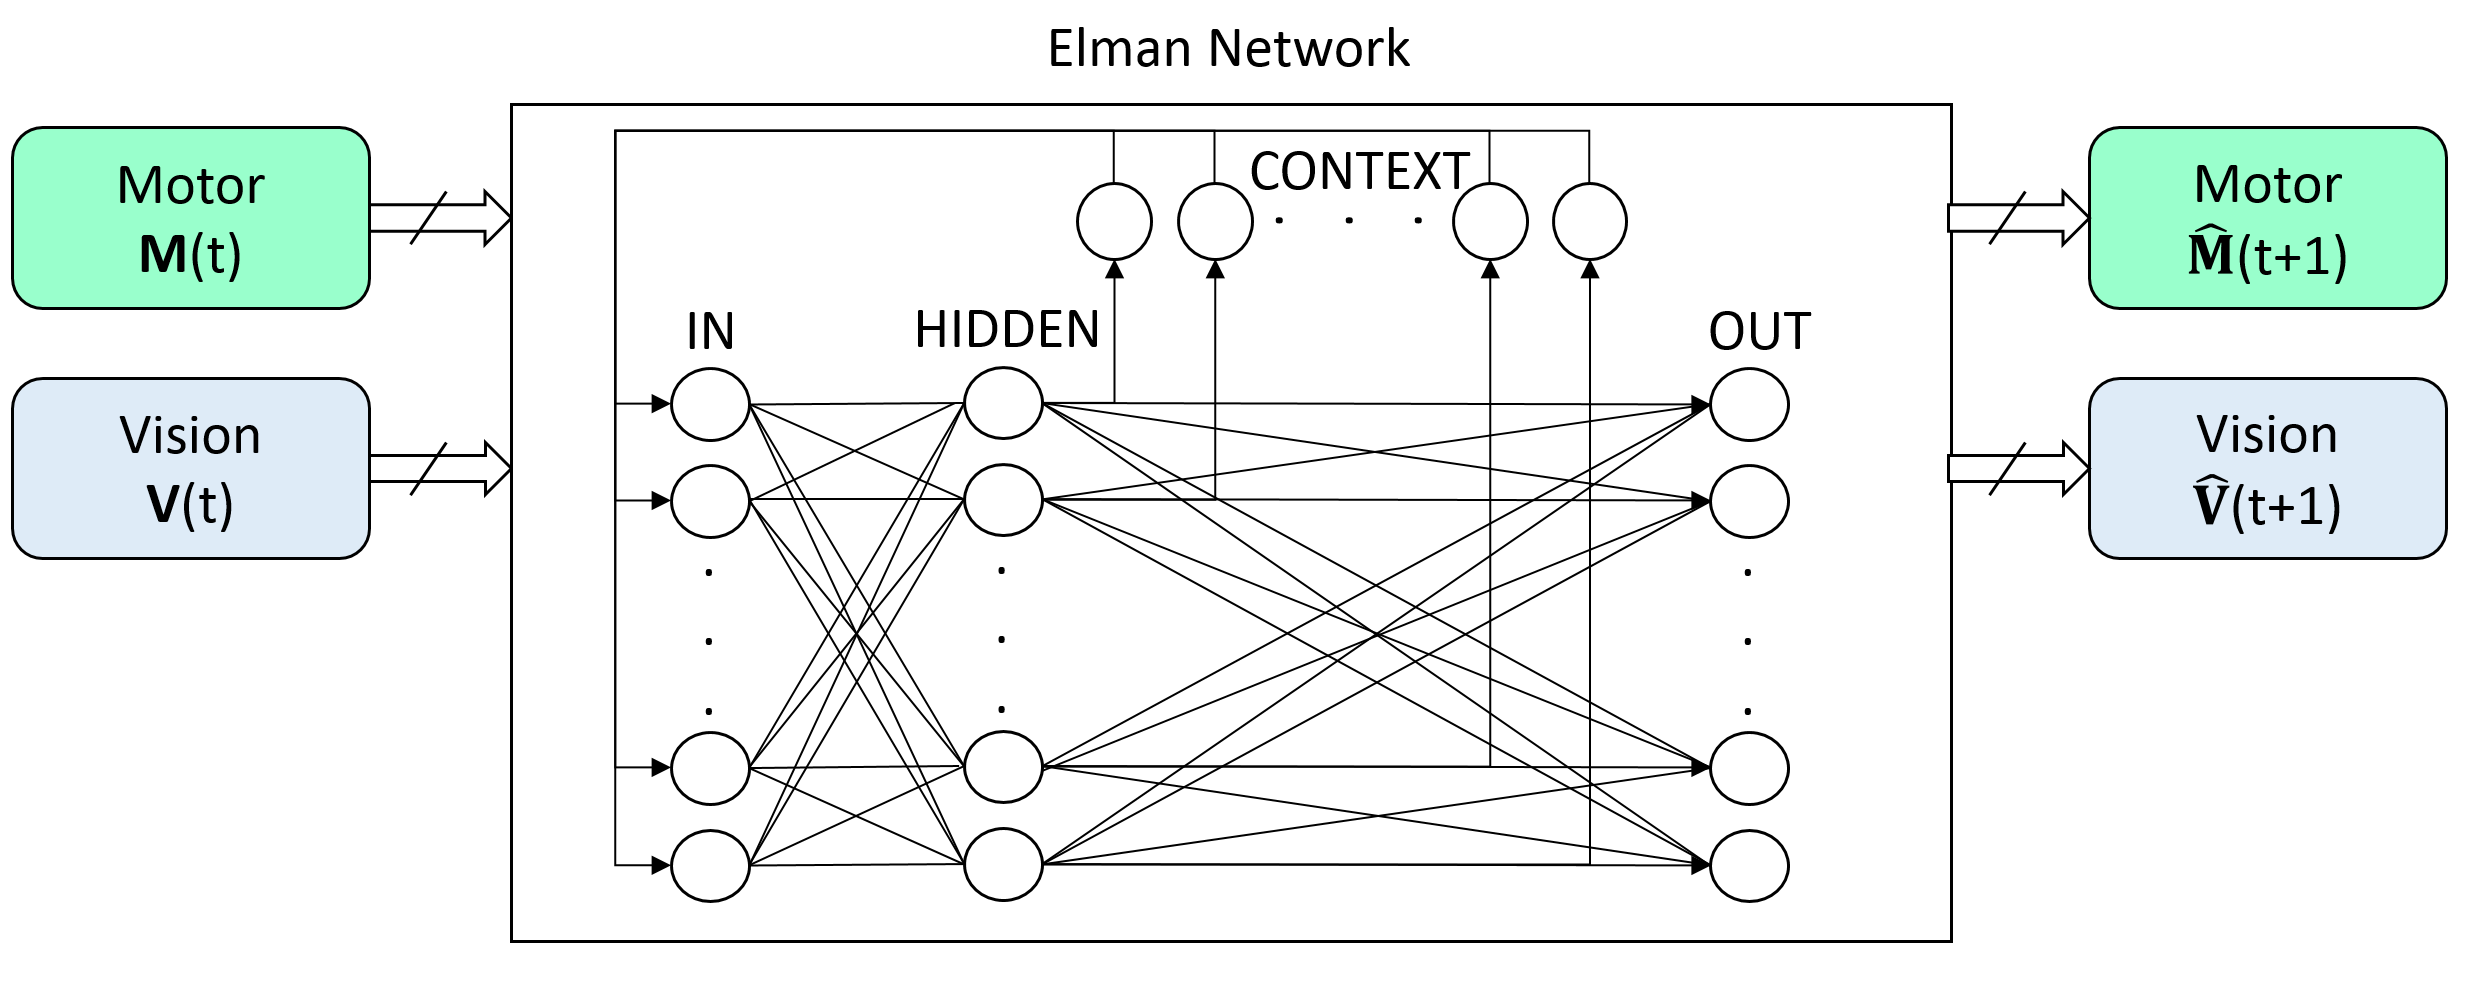
\includegraphics[width=0.5\textwidth,natwidth=700,natheight=450]{Elman_Network.png}
\caption{Internal structure of the sensorimotor integration module based on a Recurrent Neural Network}
\label{NeuralNet}
\end{figure}

\subsubsection{Prediction Error}
 Humans' capacity to make predictions is strongly influenced by their experience, and the lack of experience causes the prediction outcome to differ largely from the actual one. We define this difference as the prediction error. Here, the prediction error \(\textit{e}(t+1)\) when observing others performing an action is calculated as,

\begin{equation}
\begin{split}
	\textit{e}(t+1)=|\hat{\textbf{V}}(t+1)-\text{\textbf{V}}(t+1)|,\\
\end{split}
\end{equation}
where \(\hat{\textbf{V}}(t+1)\) is the predicted sensory data, and \(\text{\textbf{V}}(t+1)\) is the actual sensory data.

\subsection{Visual Attention Module}
For implementing the visual attention module we adopted the findings of Kidd et al. \cite{kidd2012goldilocks} who suggested that infants allocate their attention in order to maintain an intermediate level of complexity. Hereafter we will refer to this as the principle of predictability, where the complexity is represented by the prediction error. Accordingly, the visual attention is assumed to be proportional to an interest value \(\textit{q}\) (Fig. \ref{Attention}). The interest value \(\textit{q}\) is defined as follows,

\begin{equation}
  \textit{q}(t) = \frac{1}{\sigma\cdot \sqrt{2\cdot\pi}}\cdot e^{\frac{-(\textit{e}-\textit{u})^2}{2\cdot\sigma^2}}
  \label{gaussian}
\end{equation}
where \(\alpha\) is a scaling factor, \(\sigma\) is the variance and \(\textit{u}\) is the intermediate value of the prediction error, respectively. The interest function is maximized when the prediction error is moderate, that is, when the observed action is not too predictable (i.e., prediction error is low) or not too unpredictable (i.e., prediction error is high). 

\section{Experiments}

\subsection{Experimental settings}
In our experiment we reproduced similar experimental settings to those described in \cite{sommerville2005action}. This experiment procedure is summarized in Fig. \ref{experiment}. We conducted experiments with the simulated version of the humanoid robot iCub. The experiments considered two scenarios: the watch-first and the reach-first condition. For each experiment, the robot was placed 40 centimeters away of two objects, separated from each other by another 40 centimeters (see Fig. \ref{iCub}). In the watch-first scenario, the system first observed another individual reaching for one of the object from the same location as the robot. We referred to experimental settings in psychological studies that used infants' own visual perspective so they could easily find similarities between self-motion and others' motion \cite{woodward1998infants} \cite{sommerville2005action}. This phase is called the visual habituation. Then, the position of the objects was swapped and the system observed two more actions: reaching for the other object (new goal event) and reaching for the same object (new path event). In the reach-first scenario, the same process was repeated, but this time the system previously experienced reaching for both objects in the action task, before the visual habituation. The three experiments (action task, habituation and new event) were repeated 20 times with random initialization of the weights of the neural network.

\begin{figure*}
\centering
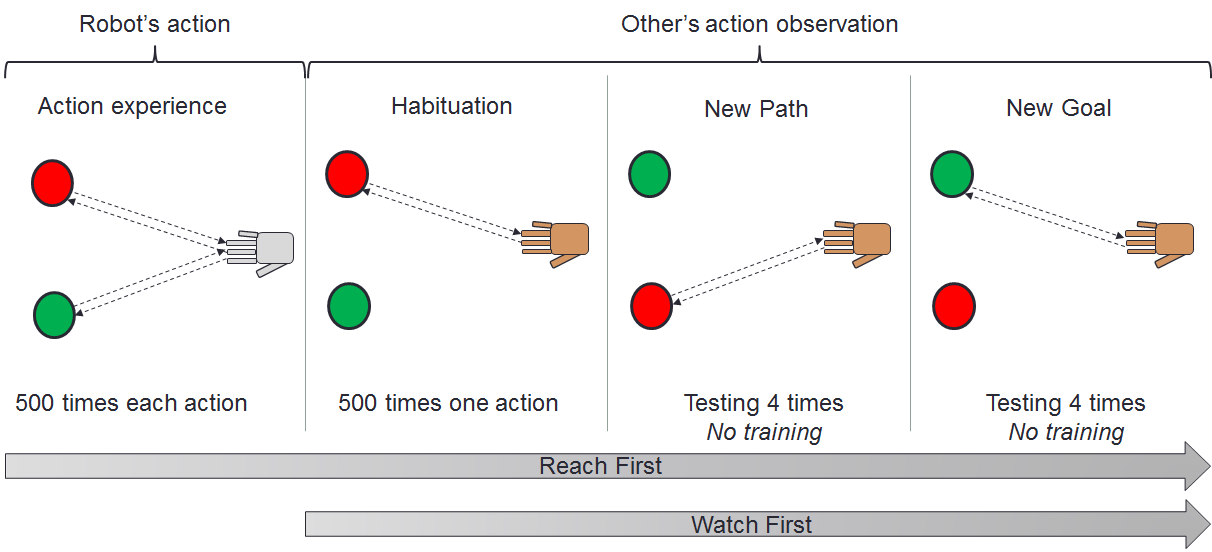
\includegraphics[width=0.76\textwidth,natwidth=700,natheight=450]{Figure2.png}
\caption{Procedure of the experiment}
\label{experiment}
\end{figure*}

\subsection{Action Task}
During the action task, the robot's arm moved toward and touched one of two objects, then came back to the initial position and repeated the same action for the same or the other object, randomly (see Fig. \ref{iCub}). This task corresponds to first stage of training for the reach-first condition, and represents accounts for the experience of coordinated visuomotor interactions. During the action task, the neural network was trained with both vision and motor data for 500 reaching actions, where each of them was composed of 175 steps (i.e., 87500 action steps). Fig. \ref{Error} (a) depicts the mean error of the action task over all training trials. The mean error \(\textit{e}_{m}\) was calculated as the average of the prediction errors in a defined time window of size $w$ = 50 (chosen empirically) in order to attenuate the noise due to the dynamic of the reaching actions, which is not the main target of this study. The mean error is defined as follows: 
\begin{equation}
	\textit{e}_{mean}(t+1) = \frac{1}{w}\sum\limits_{i=1}^{w} \textit{e}(t - i).
\end{equation}

\begin{figure}
\centering
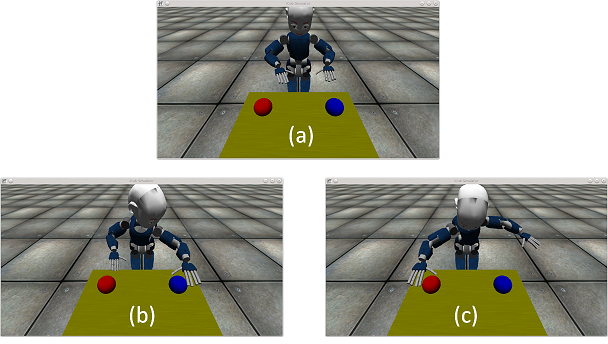
\includegraphics[width=0.40\textwidth,natwidth=700,natheight=450]{Simulator_light.png}
\caption{Experiment setting. (a): initial position before reaching; (b): reaching for object to the left of the robot; (c): reaching for object to the right of the robot.}
\label{iCub} 
\end{figure}

\subsection{Visual Habituation}
The visual habituation procedure consisted of training the neural networks with the visual data when observing others' reaching actions. Here, the neural network was the same as the one trained during the action task for the reach-first condition. Because the motor module was not used, the motor inputs were fixed to $0$ and the back-propagation was disabled for both the motor inputs and outputs so that the network does not unlearn the previously acquired motor prediction abilities (in the reach-first condition). During the habituation, the neural network was trained with only the vision for 500 reaching actions, where each of them was composed of 175 steps. Fig. \ref{Error} (b) and \ref{Error} (c) show the mean error (blue lines) for reach-first condition and watch-first condition, respectively (the initial action step between both habituation graphs differs as the action steps in reach-first condition continues from the last action step in action task). The grey curve in Fig. \ref{Error} represents the interest function (see Eq. \ref{gaussian}). In our approach, we applied straightforward the evidence in \cite{kidd2012goldilocks} which showed the visual attention shows a bell-shaped distribution in function of the error and selected a Gaussian-shaped curve to represent the interest function. Here, the intermediate error \(\textit{u}\) (Eq. \ref{gaussian}) used for the interest function \(\text{N}\) was defined as half of the maximum prediction error, where the maximum prediction error value was considered to be 0.365, which corresponded to the maximum mean error value of the condition without experience (e.g., watch-first condition). Hereafter in our discussion, the intermediate error stands as a reference to define when an error is high or low. The variance \(\sigma\) (Eq. \ref{gaussian}) was arbitrarily defined to be 0.7 for illustration purposes since it does not alter the relation between high and low errors \(\textit{e}\) and high and low interest \(\textit{q}\). Further aspects that should be considered for future works will be discussed in Section V. 

We can observe from Fig. \ref{Error} (b) and (c) that in the reach-first condition the mean error values increased in the first steps (one habituation action), and in the watch-first condition the error was high. However, the error for the reach-first condition was significantly lower than the error in the watch-first condition. This difference is due to the fact that the visual information learned during the action task in the reach-first condition contributed to keep the error relatively low. Fig. \ref{Error} also shows that the interest value (grey line) for the reach-first condition was higher than the interest value for the watch-first condition.

In relation to the findings of Sommerville et al. \cite{sommerville2005action}, these results may explain why infants in the reach-first condition looked longer to a first visual habituation compared to infants in the watch-first condition. We suggest that the coordinated visuomotor experience contributes to form a representation of own visual experience, which makes others' actions become more predictable but not fully predictable generating a prediction error that increases the visual attention.

\begin{figure}
\centering
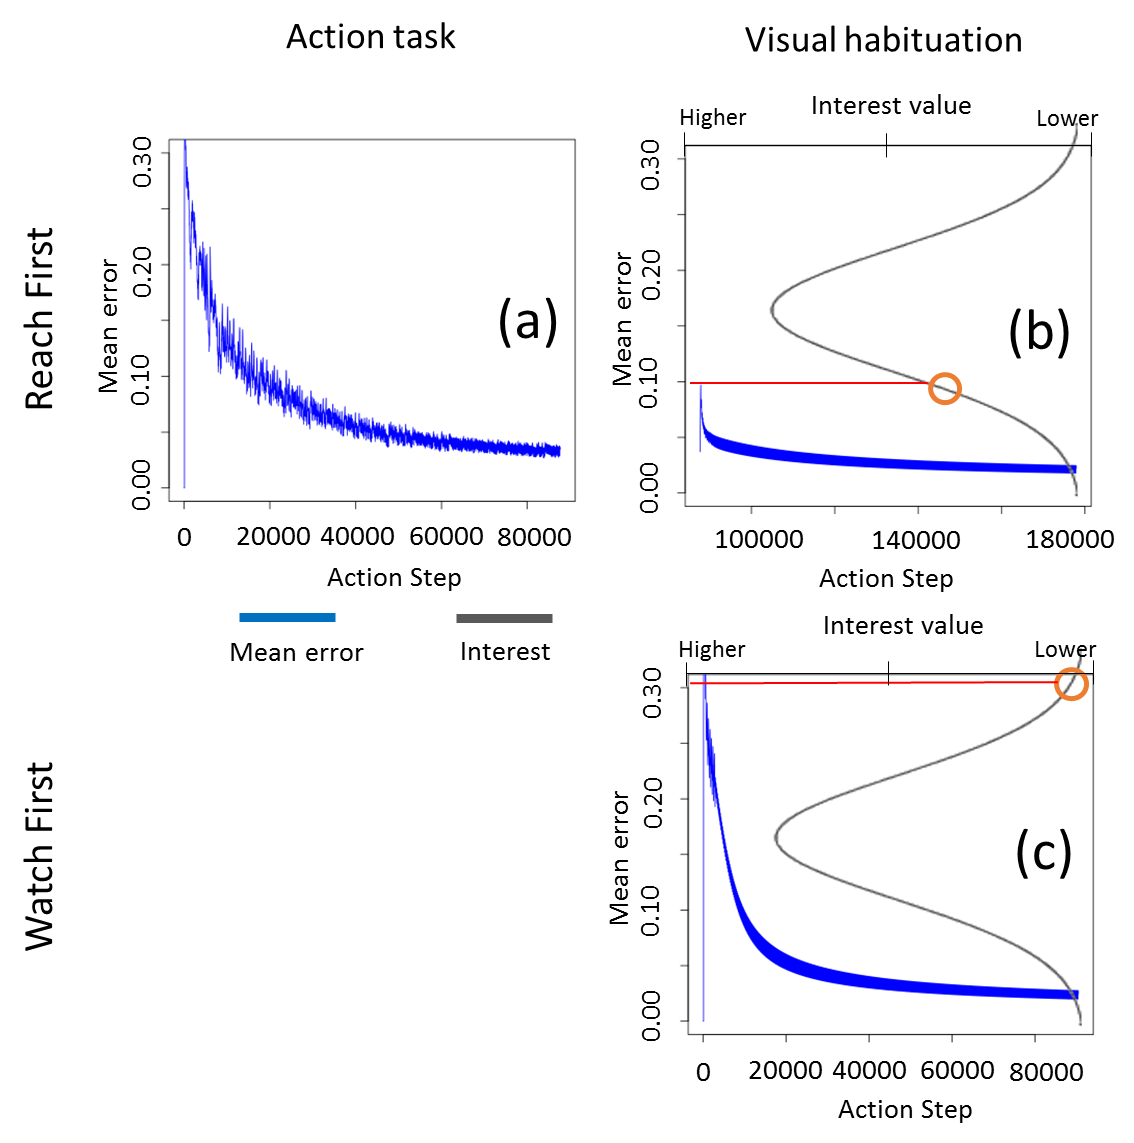
\includegraphics[width=0.5\textwidth,natwidth=700,natheight=250]{AT_HT_with_Attention_2.png}
%\includegraphics[width=0.57\textwidth,natwidth=500,natheight=300,trim=80 100 0 100]{HAB_RESULT.eps}
\caption{Training of the neural network for watch-first condition and reach-first condition. The bottom horizontal axis represents the action step, the vertical axis represents the mean error and the top horizontal axis represents the interest value. The blue line and the gray line are the mean error in function of the action step and the interest value in function of the mean error, respectively. The red line and the red point represent the intersection of the mean error with the curve of interest. (a) Mean error during action task for reach-first condition over all training trials; (b) Mean error and interest value during habituation task for reach-first condition; (c) Mean error  and interest value during habituation task for watch-first condition}
\label{Error}
\end{figure}

\subsection{New Path and New Goal}
After the networks were trained for both watch-first and reach-first conditions, we measured the mean error when the goal or the trajectory were changed respect to the original action employed during the visual habituation, namely new goal and new path event, respectively. The graphs of the mean error and the interest value for watch-first condition and reach-first condition are shown in Fig. \ref{figure7}. We can see that the change of the path or the goal produced an increase of the prediction error for all conditions, in comparison with their values in the last phase of habituation (see Fig. \ref{Error}). The results also showed that the prediction error of the system without motor experience (i.e., the watch-first condition) took distant values from the middle value of the prediction error \(\textit{u}\). However, the prediction error of the system with motor experience (i.e., the reach-first condition) took closer values to the middle value \(\textit{u}\), especially for the new goal event. Therefore, the increase of interest was higher for new goal and reach-first condition than for other conditions. 

An explanation for this result is that, in the case of watch-first condition the system learned visual trajectories ($x,y,z$) and visual relations ($r_{11}(t), r_{12}(t), r_{21}(t)$ and $r_{22}(t)$) that are specific to the targeted object in the habituation, and therefore the system produced a high prediction error for the new goal event (respect to the middle prediction error) since the system could not associate the new targeted goal, but produced a low prediction error for the new path event since the targeted object was the same. This indicates that in our experiment the visual relations had stronger effect on the prediction error than the trajectory had. Subsequently, if we compare these results to the case of the system with action experience, we can say that the experience of motor target signals ($g_{1}(t)$ and $g_{2}(t)$) allowed the system to encode action experience in terms of goals, and therefore for the new goal event the visuomotor representation analized the event not in terms of visual appearance but also in terms of the action goal. Then, the influence of the visual trajectory on prediction error got reduced, and consequently we can see that the prediction error moved from a high value in the watch-first condition to a lower value closer to the middle error in the reach-first condition.

\begin{figure}
\centering
%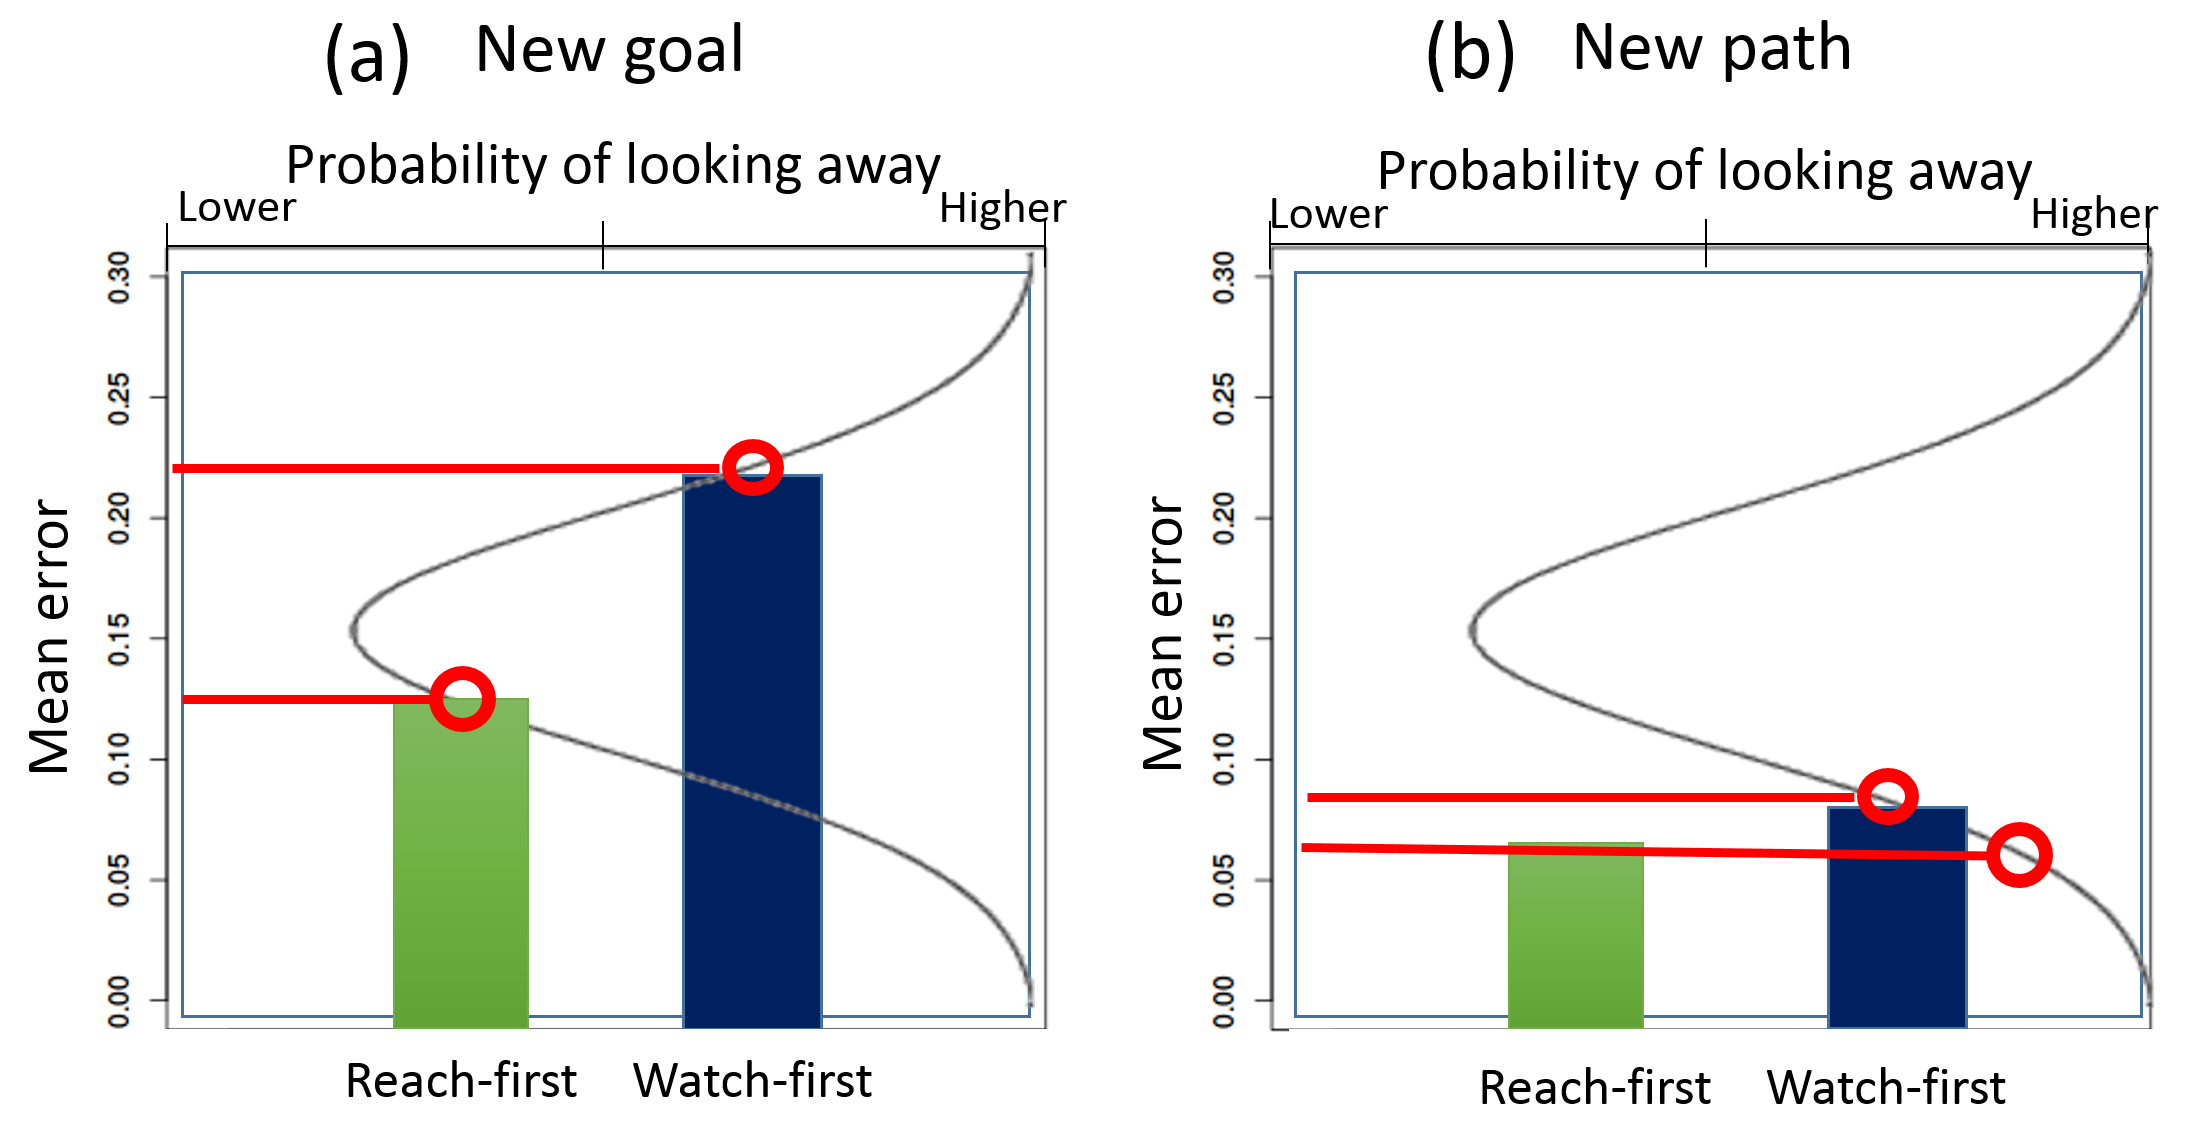
\includegraphics[width=0.5\textwidth,natwidth=700,natheight=450]{TT_with_Attention.png}
\includegraphics[width=0.45\textwidth,natwidth=300,natheight=300,trim=0 200 0 -50]{TEST_RESULT_2.eps}
%  \includegraphics[width=7cm,bb=0 0 400 500,trim=200 150 0 0]{TEST_RESULT.eps}
\caption{Error and interest during the test event. In both graphs the bottom horizontal axis represents the condition, the vertical axis represents the mean error and the top horizontal axis represents the interest function. The green and blue bars represent the mean error for the reach-first condition and the watch-first condition, respectively. The gray line, whose independent axis is the top horizontal axis, represents the interest value in function of the mean error. The red line and point represent the intersection of the mean error with the curve of interest. (a) New goal event, (b) New path event.}
\label{figure7}
\end{figure}

\section{Discussion}
Our computational approach brings significant results that may shed a light on the influence that motor experience has on the perception of others' actions. Our experimental results showed that the system acquired a joint representation of visual and motor experience of coordinated interactions  in the action task (i.e., reach-first condition), and was able to apply that visuomotor experience to make predictions of the visual and motor components of others' actions in the visual habituation. The prediction error was closer to the middle value when the system had interaction experience (i.e., reach-first condition) than when the system did not have interaction experience (i.e., watch-first condition). Our interpretation of these results is that the system with coordinated visuomotor experience associates visual experience of own actions and visual information of others' actions, which results in a moderate prediction error that stimulates an increase of visual attention.

The experiment for new path event (same goal, different path of the hand) and new goal event (different goal, same path of the hand) tested both systems (watch-first system and reach-first system) after the habituation stage when they were already familiarized with the scene. The prediction error increased for both watch-first and reach-first conditions, but the prediction error for new goal (same path) under reach-first condition was closer to the middle error, which resulted in a higher attention, similarly to the experimental results reported by Sommerville et al. \cite{sommerville2005action}. We attribute this result to the contribution of the motor component. During habituation in reach-first condition the system formed an association between its motor experience, including motion target, and the visual information of other's actions by using the joint visuomotor representation. Therefore, since the motor information encodes the goal and that information got encoded in the joint visuomotor representation, when the goal was changed the system perceived the action in terms of the goal and produced a prediction error that led to similar attention increases as those reported by \cite{sommerville2005action}. Thus, the link between our results and the psychological findings is straightforward in terms of the strong connection between motor and sensory components, and the influence that own motor experience has on visual attention.

In Fig. \ref{Error} and \ref{figure7} we presented the results including the correspondence with the visual attention based on our visual attention model. In our work we employed a Gaussian-shaped curve and the middle value of the prediction error to establish a relation between prediction error and attention allocation, and the experimental results demonstrated to be in favor of our selection. Nonetheless, we consider that tuning those parameters, including \(\sigma\) (Eq. \ref{gaussian}), still requires additional information that should be obtained by considering additional experimental conditions to those in \cite{sommerville2005action} (e.g., measuring the looking time of infants with interaction experience without gloves in the habituation phase). Here, we must highlight the importance of the results in terms of the patterns of the prediction error obtained under the different conditions. Our results demonstrated a clear influence of the motor experience on the perception reflected in the prediction error which we hypothesize ultimately alters the visual attention. Our results proved to be consistent with the perceptual changes reported by \cite{sommerville2005action}, and we consider they may constitute a significant foundation for the understanding and design of cognitive development.

\section{Conclusion}
We proposed a computational model to explain psychological findings showing that action production alters the perception of other's actions \cite{sommerville2005action}. The experimental results showed that the influence of the motor experience on the joint representation of own visuomotor experience lead to changes in perception of others' actions. Our hypothesis proved to be valid to explain main findings relating the visuomotor experience and the allocation of visual attention in infants.

As a future work, we propose analyzing the hidden layer of the neural network in order to measure the effect of the motor information in the sensorimotor representation. We believe that the prediction error play a vital role not only in visual attention allocation but also in other domains at a cognitive level. Recent psychological studies have shown that infants make distinctions between path and goal for prediction purposes \cite{cannon2012infants}. Thus, we find relevant to investigate the possible developmental connections between visual attention and prediction of others' actions.


\section*{Acknowledgment}
This work is partially supported by MEXT/JSPS KAKENHI (Research Project Numbers: 24119003, 24000012, 25700027) and JSPS Core-to-Core Program, A. Advanced Research Networks.

\bibliographystyle{ieeetr}
\bibliography{references}
\baselineskip 3.95mm

% An example of a floating figure using the graphicx package.
% Note that \label must occur AFTER (or within) \caption.
% For figures, \caption should occur after the \includegraphics.
% Note that IEEEtran v1.7 and later has special internal code that
% is designed to preserve the operation of \label within \caption
% even when the captionsoff option is in effect. However, because
% of issues like this, it may be the safest practice to put all your
% \label just after \caption rather than within \caption{}.
%
% Reminder: the "draftcls" or "draftclsnofoot", not "draft", class
% option should be used if it is desired that the figures are to be
% displayed while in draft mode.
%
%\begin{figure}[!t]
%\centering
%\includegraphics[width=2.5in]{myfigure}
% where an .eps filename suffix will be assumed under latex, 
% and a .pdf suffix will be assumed for pdflatex; or what has been declared
% via \DeclareGraphicsExtensions.
%\caption{Simulation Results}
%\label{fig_sim}
%\end{figure}

% Note that IEEE typically puts floats only at the top, even when this
% results in a large percentage of a column being occupied by floats.


% An example of a double column floating figure using two subfigures.
% (The subfig.sty package must be loaded for this to work.)
% The subfigure \label commands are set within each subfloat command, the
% \label for the overall figure must come after \caption.
% \hfil must be used as a separator to get equal spacing.
% The subfigure.sty package works much the same way, except \subfigure is
% used instead of \subfloat.
%
%\begin{figure*}[!t]
%\centerline{\subfloat[Case I]\includegraphics[width=2.5in]{subfigcase1}%
%\label{fig_first_case}}
%\hfil
%\subfloat[Case II]{\includegraphics[width=2.5in]{subfigcase2}%
%\label{fig_second_case}}}
%\caption{Simulation results}
%\label{fig_sim}
%\end{figure*}
%
% Note that often IEEE papers with subfigures do not employ subfigure
% captions (using the optional argument to \subfloat), but instead will
% reference/describe all of them (a), (b), etc., within the main caption.


% An example of a floating table. Note that, for IEEE style tables, the 
% \caption command should come BEFORE the table. Table text will default to
% \footnotesize as IEEE normally uses this smaller font for tables.
% The \label must come after \caption as always.
%
%\begin{table}[!t]
%% increase table row spacing, adjust to taste
%\renewcommand{\arraystretch}{1.3}
% if using array.sty, it might be a good idea to tweak the value of
% \extrarowheight as needed to properly center the text within the cells
%\caption{An Example of a Table}
%\label{table_example}
%\centering
%% Some packages, such as MDW tools, offer better commands for making tables
%% than the plain LaTeX2e tabular which is used here.
%\begin{tabular}{|c||c|}
%\hline
%One & Two\\
%\hline
%Three & Four\\
%\hline
%\end{tabular}
%\end{table}


% Note that IEEE does not put floats in the very first column - or typically
% anywhere on the first page for that matter. Also, in-text middle ("here")
% positioning is not used. Most IEEE journals/conferences use top floats
% exclusively. Note that, LaTeX2e, unlike IEEE journals/conferences, places
% footnotes above bottom floats. This can be corrected via the \fnbelowfloat
% command of the stfloats package.








% trigger a \newpage just before the given reference
% number - used to balance the columns on the last page
% adjust value as needed - may need to be readjusted if
% the document is modified later
%\IEEEtriggeratref{8}
% The "triggered" command can be changed if desired:
%\IEEEtriggercmd{\enlargethispage{-5in}}

% references section

% can use a bibliography generated by BibTeX as a .bbl file
% BibTeX documentation can be easily obtained at:
% http://www.ctan.org/tex-archive/biblio/bibtex/contrib/doc/
% The IEEEtran BibTeX style support page is at:
% http://www.michaelshell.org/tex/ieeetran/bibtex/
%\bibliographystyle{IEEEtran}
% argument is your BibTeX string definitions and bibliography database(s)
%\bibliography{IEEEabrv,../bib/paper}
%
% <OR> manually copy in the resultant .bbl file
% set second argument of \begin to the number of references
% (used to reserve space for the reference number labels box)
%\begin{thebibliography}{1}

%\bibitem{IEEEhowto:kopka}
%H.~Kopka and P.~W. Daly, \emph{A Guide to \LaTeX}, 3rd~ed.\hskip 1em plus
% 0.5em minus 0.4em\relax Harlow, England: Addison-Wesley, 1999.

%\end{thebibliography}




% that's all folks
\end{document}


